
\section{Background and motivations}
\label{sec:background}

\begin{figure*}
\centering
\begin{tikzpicture}
\matrix (m) [matrix of math nodes,row sep=4em,column sep=4em] {
\node(ss)[draw]{signaling}; & \node(p3)[draw]{p3}; \\
\node(p1)[draw]{p1}; & \node(p2)[draw]{p2}; \\
};
\path[->]
  (p2) edge[dashed] node[fill=white]{1:emit} (ss)
  (p3) edge[dashed] node[fill=white,bend left]{2:pull} (ss)
  (p3) edge[dashed, bend right] node[fill=white]{3:accept} (ss)
  (p2) edge[dashed,bend left] node[fill=white]{4:pull} (ss)
  (p3) edge[<->,thick] node[fill=white,right]{5:connected} (p2);
\end{tikzpicture}%
\begin{tikzpicture}
\matrix (m) [matrix of math nodes,row sep=4em,column sep=4em] {
\node(ss)[draw]{signaling}; & \node(p3)[draw]{p3}; \\
\node(p1)[draw]{p1}; & \node(p2)[draw]{p2}; \\
};
\path[->]
  (p1) edge[dashed,bend left] node[fill=white]{1:emit} (p2)
  (p2) edge[dashed,bend left] node[fill=white,left]{2:emit/p1} (p3)
  (p3) edge[dashed,bend left] node[fill=white,right]{3:accept/p1} (p2)
  (p2) edge[dashed,bend left] node[fill=white]{4:accept} (p1)
  (p1) edge[<->,thick] (p2)
%  (p1) edge[<->,thick,bend left] (p3)
  (p2) edge[<->,thick]  (p3);

\end{tikzpicture}%
\begin{tikzpicture}
\matrix (m) [matrix of math nodes,row sep=4em,column sep=4em] {
\node(ss)[draw]{signaling}; & \node(p3)[draw]{p3}; \\
\node(p1)[draw]{p1}; & \node(p2)[draw]{p2}; \\
};
\path[->]
  (p1) edge[<->,thick] (p2)
  (p1) edge[<->,thick] (p3)
  (p2) edge[<->,thick]  (p3);
\end{tikzpicture}


\end{figure*}
WebRTC is able to establish a data channel between two browsers even
with complex network settings such as firewall, proxies or Net Address
Translation (NAT). Nevertheless, the connection establishment protocol
differs from traditional setting: it uses a three-way handshake
connection set up.  Thus, a subscription message must be
\begin{inparaenum}[(1)]
\item emitted at Peer $p$,
\item accepted at Peer $q$,
\item completed at Peer $p$.
\end{inparaenum}
  
Therefore, when a peer needs to establish a connection to another
peer, a message must travel back and forth. One could use a dedicated
server to establish the necessary dialog~\cite{peerjs}. However, this
solution does not scale considering the fact that each peer in the
network must dynamically create and remove connections over time. On
the other hand, using the built network itself distributes the load of
these connections establishment among the members.

\begin{asparadesc}
\item [Scamp]\cite{ganesh2001scamp,ganesh2003peer} stands for SCalable
  Membership Protocol. This protocol links each membership event with an
  appropriate reaction.  The most important event is the joining event which
  creates a logarithmically increasing number of connections compared to the
  total network size. The resulting graph is connected. However, the newest
  peers have few elements in their partial view, and the older peers are more
  likely clustered. Thus it needs a balancing protocol.

  In the WebRTC context, the issue of \SCAMP{} lies in the fact that the
  subscription mechanism can create connections several hops away from its
  origin (cf. Figure~\ref{fig:handshakeexample}). Unfortunately each of these
  hops is an opportunity of failure. Let $P_f$ the probability of either the
  peer or the link between the latter and the next peer crashes/disconnects
  when it holds the subscription, without possible recovery. Let $P_E$ the
  probability that a connection establishment cannot be completed. Without
  three-way handshake, $P_E$ is straightforward:
  \begin{equation} P_{E,\,1way}^{Scamp}=1-(1- P_f)^{k+1} \end{equation} where
  $k$ is the number of hops before the acceptance of the subscription, i.e.,
  there are $2$ hops at least. Indeed, the first peer cannot directly accept
  the subscription. On the other hand, in the handshaking context, the
  subscription must travel back to its origin in order to be completed. As
  consequence, when a subscription travels through a peer or a link, they are
  not allowed to fail until the subscription travels back. Thus, we obtain:
  \begin{align} P_{E,\,3way}^{Scamp} &=1 - ((1-P_f)^{2(k+1)} (1-P_f)^{2k}
                                       \ldots (1-P_f)^2) \nonumber \\
                                     &=1-(1-P_f)^{k^2+3k+2}
  \end{align}
  The complexity class of the \SCAMP{} failure rate under three-way handshake
  increases. Thus, it does not scale in number of peers any more.
\end{asparadesc}


\begin{asparadesc}
\item [Random peer sampling] protocols~\cite{jelasity2004peer} provide each
  peer with a partial view $\mathcal{P}$ of the network membership
  $\mathcal{N}$. They populate the partial views with peers chosen at random
  among $\mathcal{N}$ following a uniform distribution using local knowledge
  only. They aim to converge to a random graph, hence, providing connectedness,
  robustness and efficient epidemic spreading of messages. A wide variety of
  gossip-based protocols use random peer sampling (e.g. topology
  management~\cite{voulgaris2005epidemic, jelasity2009tman,dabek2004vivaldi}).
  Our \SCAMPLON{} protocol is inspired by two state-of-the-art approaches,
  namely \SCAMP{} and \CYCLON{}.
\end{asparadesc}

\begin{asparadesc}
\item [Cyclon]\cite{voulgaris2005cyclon} is a periodic random peer sampling
  protocol which updates its partial view every interval of time. The partial
  view has a fixed-size set at start. In this view, each neighbor is
  associated with an age incremented at each cycle. To update its partial view,
  \CYCLON{} exchanges a subset of its partial view with one of its neighbor
  chosen using the age.  Assuming a well chosen $|\mathcal{P}|$, \CYCLON{}
  quickly converges to a random graph and quickly withdraws crashed/left peers.

  In the WebRTC context, each connection matters. Hence, we cannot afford
  oversized partial views like in \CYCLON{}. For instance, considering an
  application usable by small or large groups of users indifferently, \CYCLON{}
  will overestimate to adapt to the largest groups. While this is indeed
  required for these latter, the small groups of users will suffer of increased
  traffic (oversized partial views maintenance, increased redundancy during the
  broadcast of messages). If the group is small enough, the graph could be
  fully connected which is highly undesirable.
\end{asparadesc}


\begin{problem}
  Let $t$ be an arbitrary time frame, let $\mathcal{N}^t$ be the network
  membership at that given time $t$ and let $\mathcal{P}_x^t$ be the partial view of peer $p_x \in \mathcal{N}^t$. 
  A cost-efficiant random peer sampling, especially when three-way handshaking is
  involved, should provide the following best-case properties:
  \begin{center}
    Partial view size: \hfill
    $\forall p_x \in \mathcal{N}^t,\, |\mathcal{P}_x^t| = \Theta (\ln
    |\mathcal{N}^t|)$
  \end{center}
  \begin{center}
    Time complexity of a connection: \hfill $O(1)$
  \end{center}
  \begin{center}
    Convergence speed: \hfill $\Theta(\exp \, t^{-1})$
  \end{center}
\end{problem}

\begin{figure}
  \centering
  
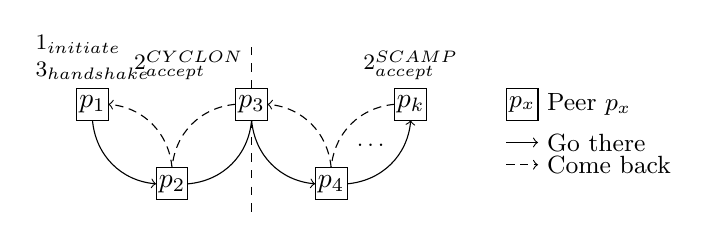
\begin{tikzpicture}[scale=1.15]

  \footnotesize
  \draw (0pt,5pt)node[align=left,anchor=south]{$1_{initiate}$\\
    $3_{handshake}$};
  \draw (50pt, 5pt)node[anchor=south east]{$2_{accept}^{CYCLON}$};
  \draw (100pt,5pt)node[anchor=south]{$2_{accept}^{SCAMP}$};
  \draw (88pt, -13pt)node{\ldots};

  \draw[dashed](50pt,-5pt)--(50pt,-35pt);
  \draw[dashed](50pt, 5pt)--(50pt, 20pt);

  \normalsize
  \draw[fill=white] (0pt, 0pt) node{$p_1$} +(-5pt,-5pt) rectangle +(5pt,5pt);
  \draw[fill=white] (25pt,-25pt) node{$p_2$} +(-5pt,-5pt) rectangle +(5pt,5pt);
  \draw[fill=white] (50pt, 0pt) node{$p_3$} +(-5pt,-5pt) rectangle +(5pt,5pt);
  \draw[fill=white] (75pt,-25pt) node{$p_4$} +(-5pt,-5pt) rectangle +(5pt,5pt);
  \draw[fill=white] (100pt, 0pt) node{$p_k$} +(-5pt,-5pt) rectangle +(5pt,5pt);


  \draw[->] ( 0pt,-5pt) to[out=-85,in=175] (20pt,-25pt);
  \draw[->, densely dashed] (25pt, -20pt) to[out=95,in=-5] ( 5pt, 0pt);
  \draw     ( 30pt, -25pt) to[out=5,in=-95] (50pt,-5pt);
  \draw[densely dashed] ( 45pt, 0pt) to[out=185,in=85] (25pt, -20pt);
  \draw[->] (50pt, -5pt) to[out=-85,in=175] (70pt,-25pt);
  \draw[->, densely dashed] (75pt, -20pt) to[out=95,in=-5] (55pt,0pt);
  \draw[->] (80pt, -25pt) to[out=5pt,in=-95] (100pt,-5pt);
  \draw[densely dashed] (95pt, 0pt) to[out=185,in=85] (75pt, -20pt);
%%  \draw[->, densely dashed] (-70pt, 0pt) -- (-30pt, 0pt); %% u1 -> u4
%%  \draw[->, densely dashed] (-5pt, 30pt) -- (-70pt, 5pt); %% u3 -> u1
%%  \draw[->, densely dashed] (30pt, -5pt) to[out=-85,in=-95](-70pt,-5pt);%%u5 u1

  \small 
  \begin{scope}[shift={(130pt,0pt)}]
    \draw[fill=white](5pt, 0pt)node{$p_x$}+(-5pt,-5pt) rectangle +(5pt,5pt);
    \draw (10pt,0pt) node[anchor=west]{Peer $p_x$};
    \draw[->](0pt, -12pt)--(10pt, -12pt) node[anchor=west]{Go there};
    \draw[->, densely dashed](0pt, -19pt)--(10pt, -19pt)
    node[anchor=west]{Come back};    
  \end{scope}
  
\end{tikzpicture}
  \caption{\label{fig:handshakeexample}Handshaking differences of \CYCLON{} and
    \SCAMP{}. While subscriptions travel from $p_1$ to $p_3$ using one
    intermediate in \CYCLON{}, the subscriptions travel from $p_1$ to $p_k$ in
    \SCAMP{}. This difference change the complexity of the two approaches. In
    particular, the failure probability is much more important in
    \SCAMP{}. Indeed, links and peers, once employed, must be kept alive until
    the subscriptions travel back. Otherwise, the handshaking cannot be
    completed.}
\end{figure}

Unfortunately, while the properties of both approaches converge exponentially fast
to those of a random graph, each of them fails either on the partial view size requirement
(i.e. \CYCLON{}) or the time complexity of connection establishment
(i.e. \SCAMPLON{}). Knowingly, we would like the best of the aforementioned
approaches in order to answer to the problem statement. Ultimately, it would
allow cost-efficient gossiping on top of WebRTC. Hence, it would open the gate to a wide
variety of distributed and decentralized applications requiring a scalable
broadcast.

%%% Local Variables:
%%% mode: latex
%%% TeX-master: "../paper"
%%% End:
